\chapter{Background}\label{chap:background}
Some background knowledge is necessary for the reader to have an understanding of the principles behind semantic segmentation and convolutional neural networks.
This chapter on the background of this work will discuss semantic segmentation, machine learning with artificial neural networks and convolutional neural networks, curb segmentation, loss functions, network optimizers, and binary dilation.

\section{Semantic Segmentation}\label{section:background-segmentation}
Unlike image classification, which classifies the contents of an image as a whole, semantic segmentation is the use of some algorithm to process an image and assign class labels to each individual pixel~\cite{segmentation-medium}.
This adds the ability to locate and classify multiple objects in a given scene.
For example, the ground truth segmentation of the street-level image in \figref{fig:background-raw} can be seen in \figref{fig:background-segmented}.
Each pixel of the image has been assigned a class, which is represented by the different colors in the segmented image.
This allows a computer or program to understand what objects are in the image it is shown.

\begin{figure}
    \centering
    \begin{subfigure}{0.45\textwidth}
    	\centering
    	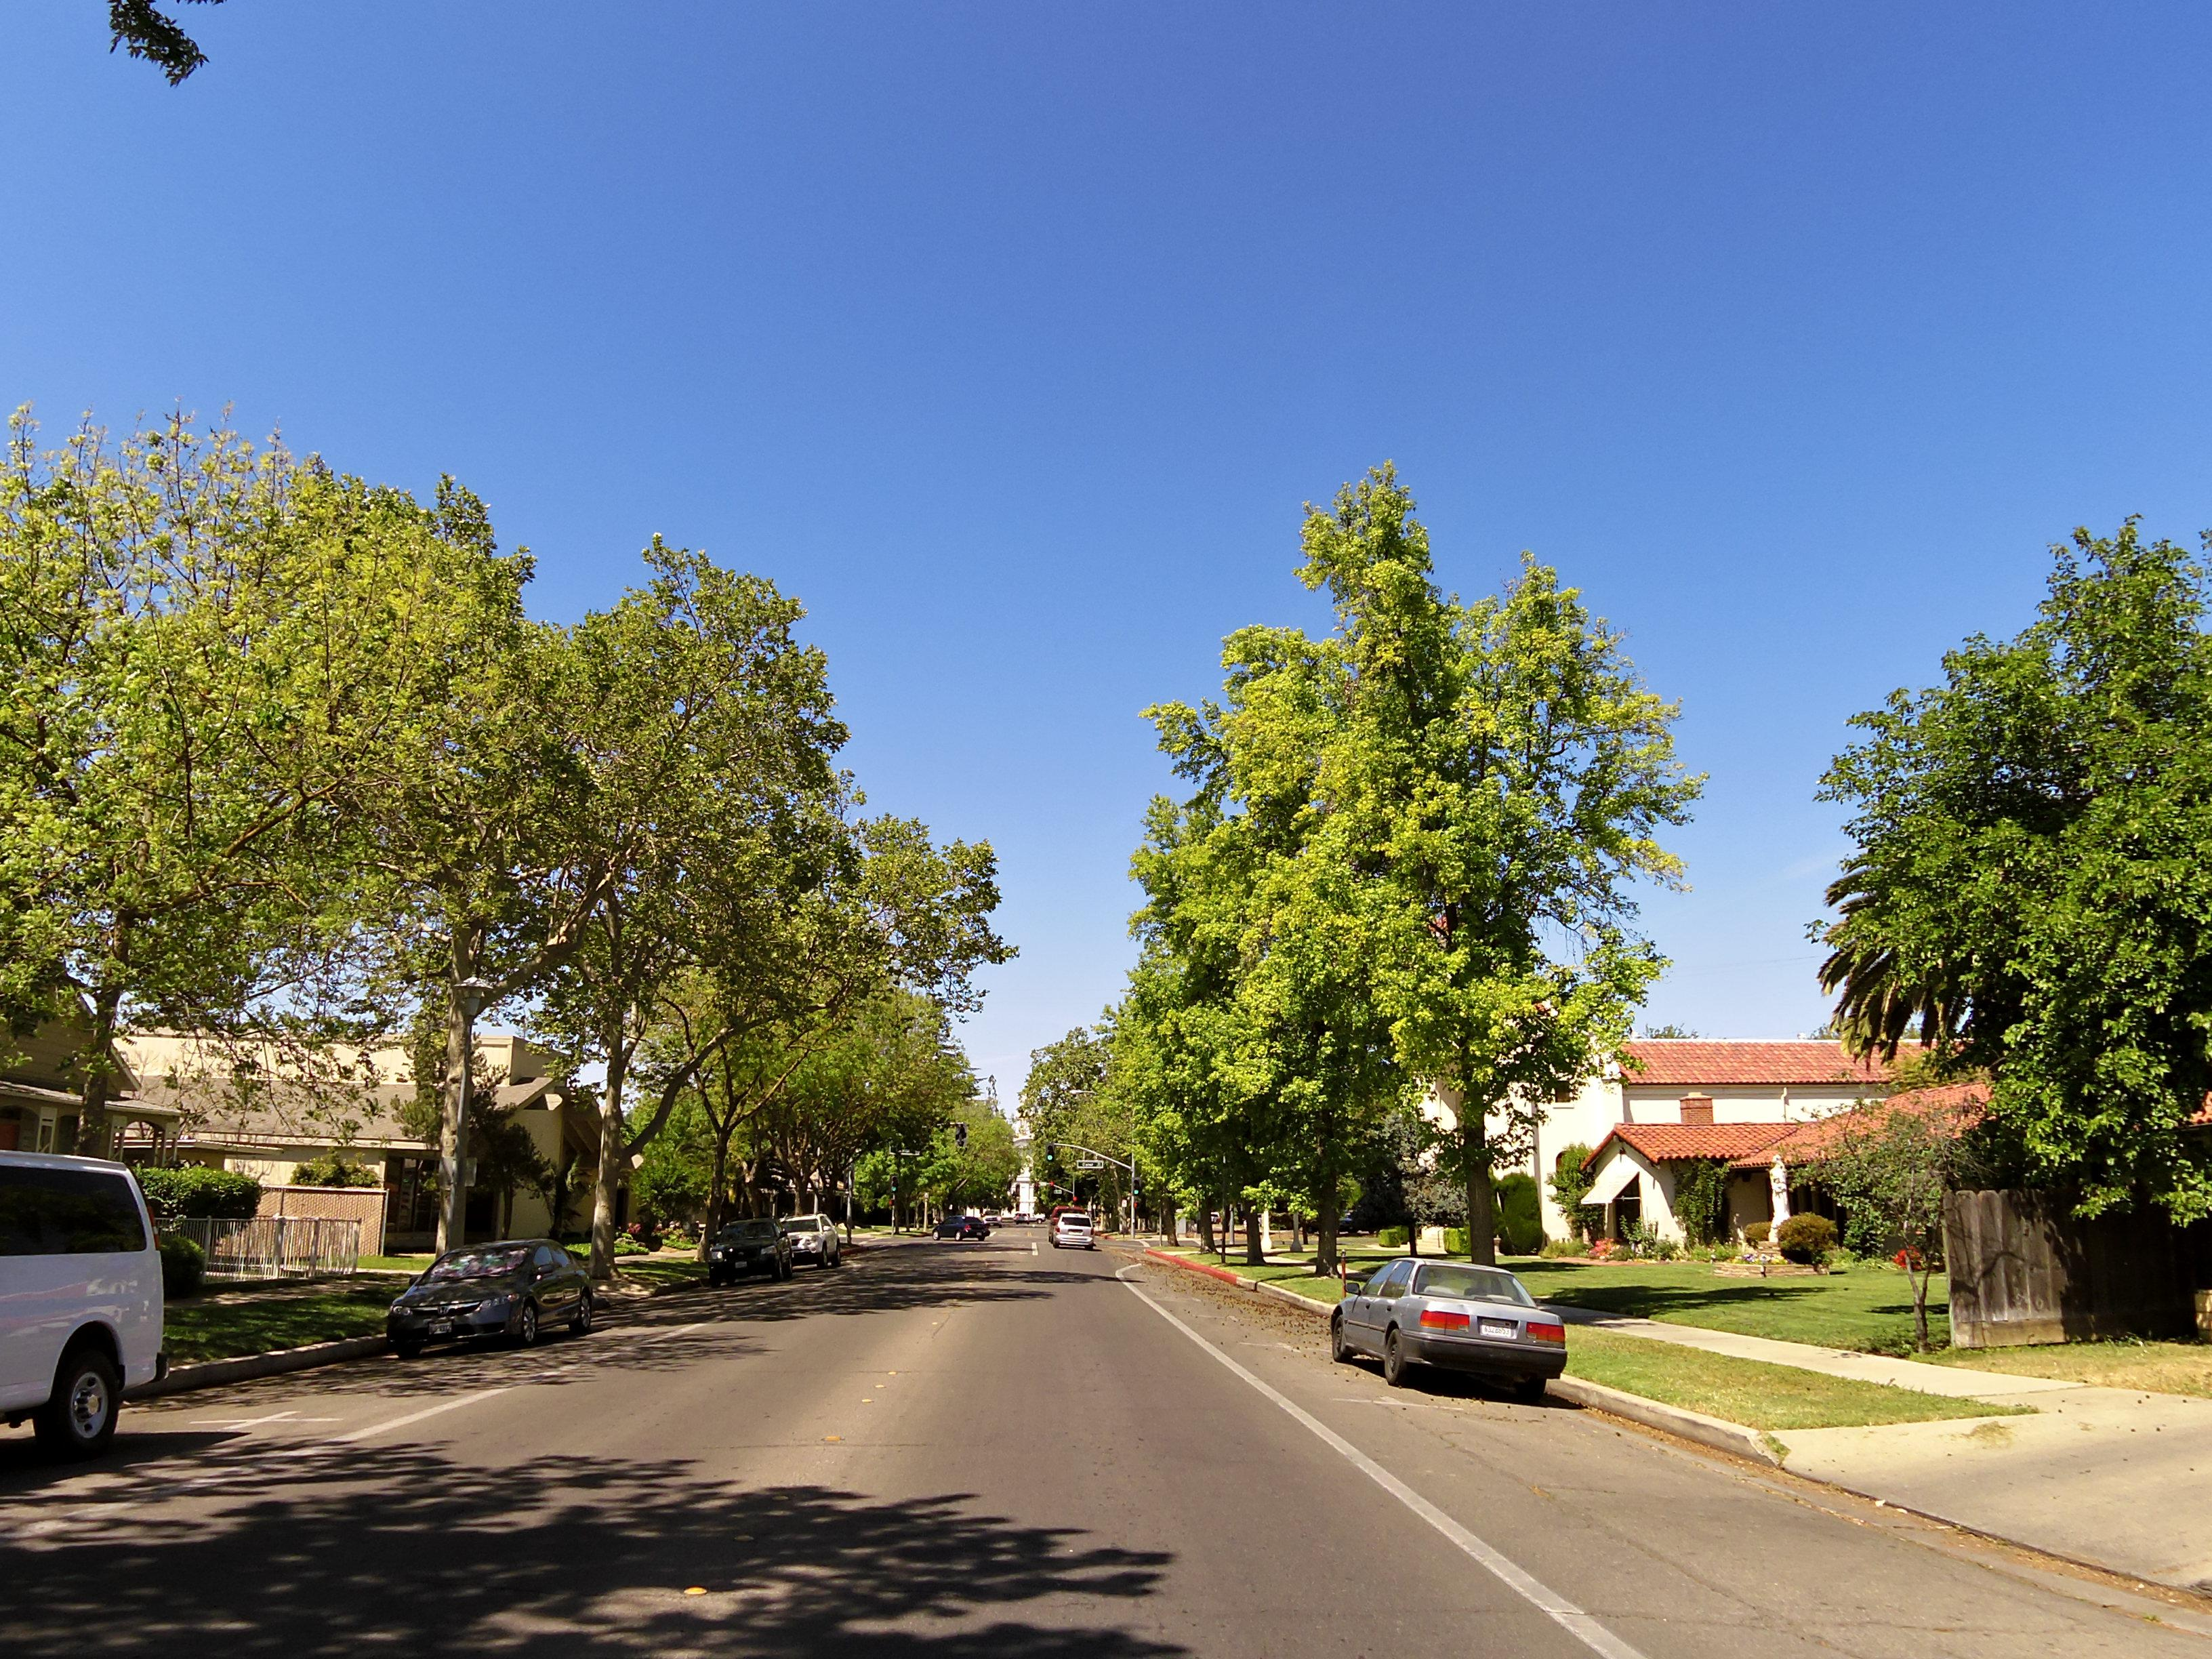
\includegraphics[width=0.9\textwidth]{figures/background/raw.jpg} % first figure itself
    	\caption{An example of a street-level image that is taken using a regular color camera.} \label{fig:background-raw}
    \end{subfigure}
	\hfill
    \begin{subfigure}{0.45\textwidth}
        \centering
        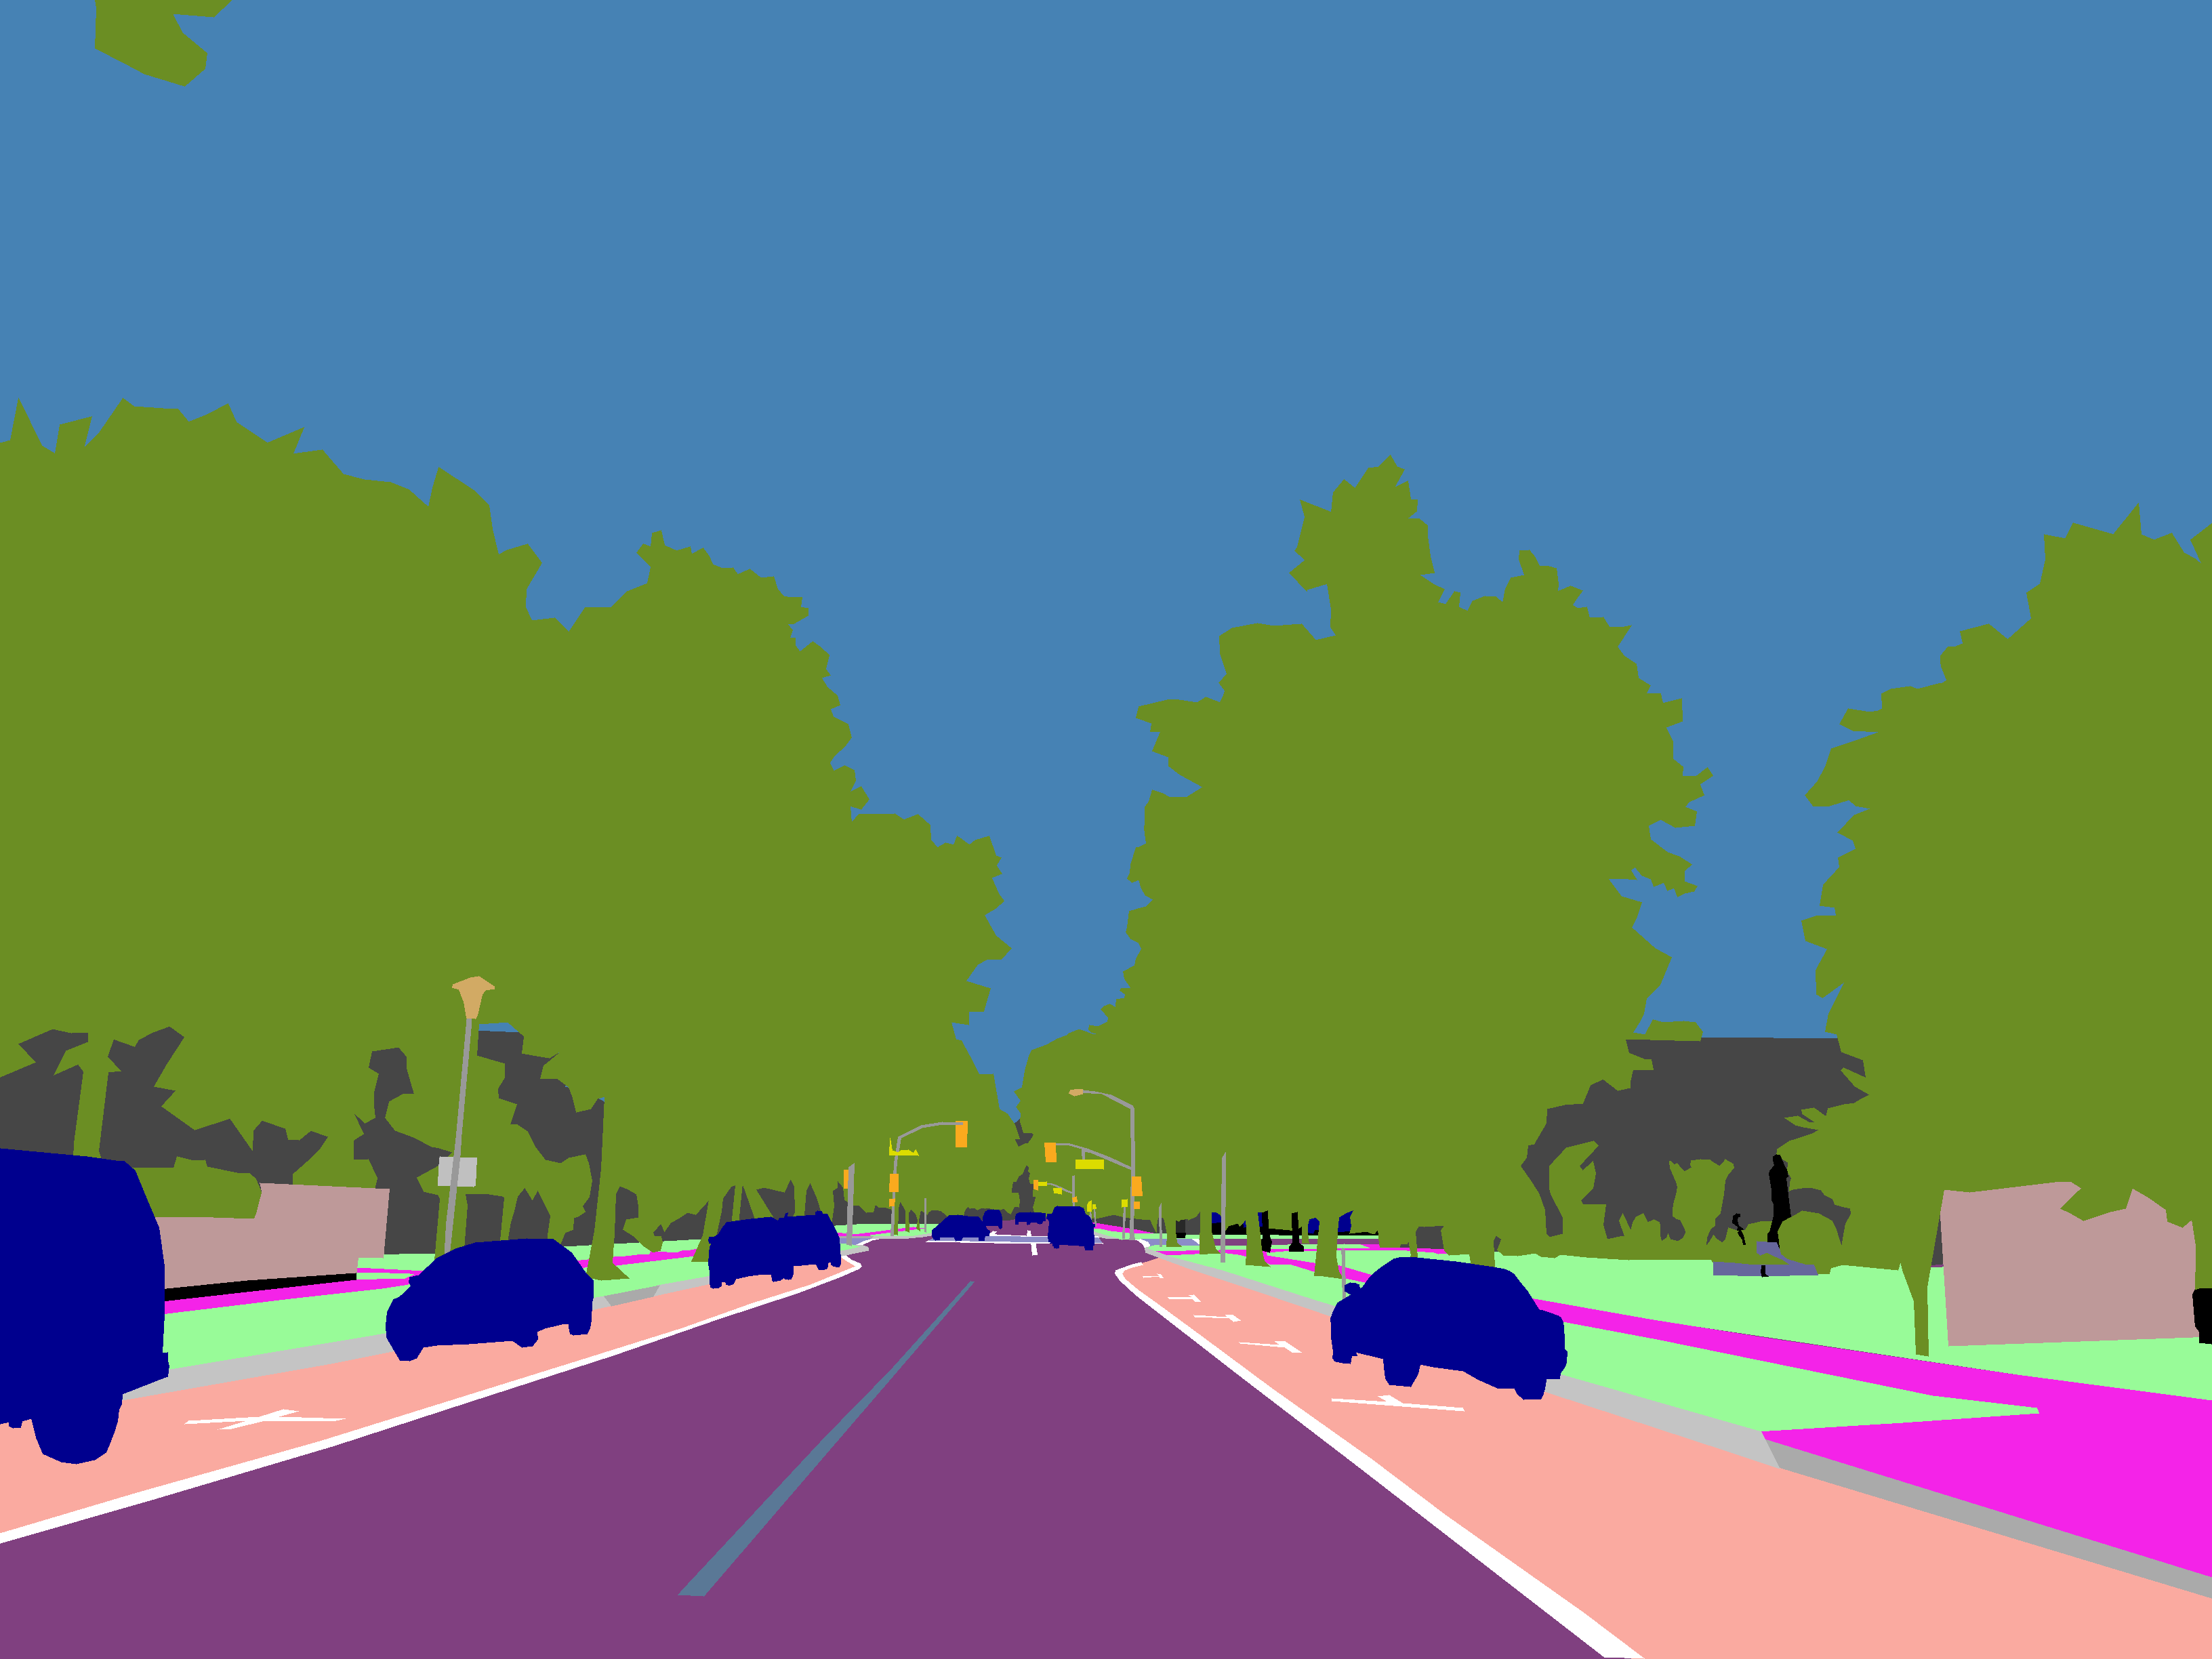
\includegraphics[width=0.9\textwidth]{figures/background/segmented.png} % second figure itself
        \caption{The segmented version of the image, each color representing a different class.} \label{fig:background-segmented}
    \end{subfigure}
	\caption[An example of semantic segmentation.]{An example of semantic segmentation on a color image. This example is taken from the Mapillary dataset~\cite{mapillary}.}
\end{figure}

By segmenting an image in this way, the program can interpret the scene semantically.
For example, by receiving the segmented image, a program can identify that there are line markings on the road and that there is a vehicle in front of it.
The segmentation of images in this way is essential in many robotic applications as it allows further higher level processing of the scene.

Towards the goal of this work, the segmentation of traversability classes in a scene allows Obelix to more accurately find a path allowing for the safe traversal from sidewalk to street level via curb cuts.

\section{Artificial Neural Networks}
Artificial neural networks are a computing system inspired by biological neurons. Neural networks are comprised of neurons which are capable of taking any number of numerical inputs and outputs a numerical value.

\tikzset{%
	every neuron/.style={
		circle,
		draw,
		minimum size=1cm
	},
	neuron missing/.style={
		draw=none, 
		scale=4,
		text height=0.333cm,
		execute at begin node=\color{black}$\vdots$
	},
}

\begin{figure}[t]
	\centering
	\resizebox{0.6\textwidth}{!}{
		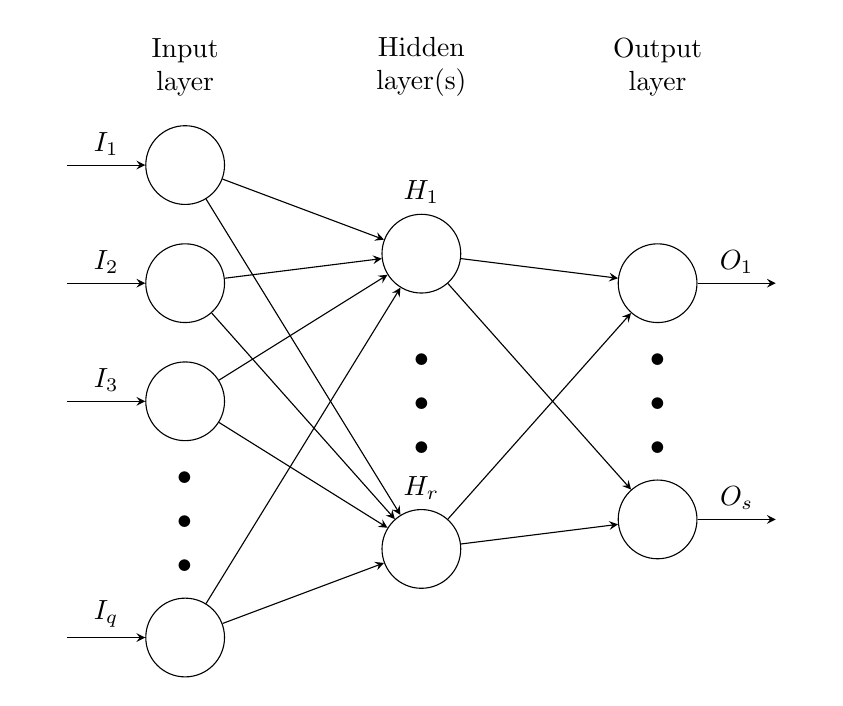
\begin{tikzpicture}[x=1.5cm, y=1.5cm, >=stealth]
			% Input neurons
			\foreach \m/\l [count=\y] in {1,2,3,missing,4}
			  \node [every neuron/.try, neuron \m/.try] (input-\m) at (0,2.5-\y) {};
			% Hidden neurons
			\foreach \m [count=\y] in {1,missing,2}
			  \node [every neuron/.try, neuron \m/.try ] (hidden-\m) at (2,2-\y*1.25) {};
			% Output neurons
			\foreach \m [count=\y] in {1,missing,2}
			  \node [every neuron/.try, neuron \m/.try ] (output-\m) at (4,1.5-\y) {};
			% Input labels
			\foreach \l [count=\i] in {1,2,3,q}
			  \draw [<-] (input-\i) -- ++(-1,0)
			    node [above, midway] {$I_\l$};
			% Hidden neuron labels
			\foreach \l [count=\i] in {1,r}
			  \node [above] at (hidden-\i.north) {$H_\l$};
			% Out arrows with labels
			\foreach \l [count=\i] in {1,s}
			  \draw [->] (output-\i) -- ++(1,0)
			    node [above, midway] {$O_\l$};
			% Input to hidden arrows
			\foreach \i in {1,...,4}
			  \foreach \j in {1,...,2}
			    \draw [->] (input-\i) -- (hidden-\j);
			% Hidden to output arrows
			\foreach \i in {1,...,2}
			  \foreach \j in {1,...,2}
			    \draw [->] (hidden-\i) -- (output-\j);
			% Layer labels
			\node [align=center, above] at (0,2) {Input \\ layer};
			\node [align=center, above] at (2,2) {Hidden \\ layer(s)};
			\node [align=center, above] at (4,2) {Output \\ layer};
		\end{tikzpicture}
	}
	\caption[Artificial Neural Networks]{A Visualization of how neurons interact within an artificial neural network. In this example, the network has 3 layers: An input layer, a hidden layer, and an output layer. The input layer consists of $q$ neurons, each having one input value. Each of these inputs neurons are connected to each of the $r$ neuron in the hidden layer. Each neuron in the hidden layer is also connected to each neuron in the output layer. Finally, the output layer contains $s$ neurons and returns $s$ output values.}\label{fig:background-neuralnet}
\end{figure}

Mathematically, a single neuron is a function.
The function of a neuron $j$ receiving input $x_j$ and producing output $y_j$ is composed of the activation $a_j$, an activation function $f_a$ which returns the activation, and an output function $f_{o}$.
The activation $a_j$ can also be considered the neuron's state.
The activation function $f_a$ calculates $a_j$ given the network input $x_j$ and can be defined as:
\begin{align}
	a_j &= f_a\left(x_j\right)
\end{align}
The output function $f_o$ computes $y_j$ based on $a_j$ and is defined as:
\begin{align}
	x_j &= f_o\left(a_j\right)
\end{align}
Many activation functions exists and are used including the identity function and the rectified linear unit (ReLU), defined as:
\begin{align}
	f_a(x) &= 
	\begin{cases}
		0	& \text{for } x \leq 0\\
		x	& \text{for } x > 0
	\end{cases}
\end{align}

Between each neuron in the network are connections which transfer the output of neuron $i$ to neuron $j$. Each of these connections are assigned a weight $w_{ij}$, which is computed by the learning algorithm.
Each neuron also has a bias $w_{0j}$.
These parameters are used to provide a neuron its input $x_j$. This is defined as:
\begin{align}
	x_j &= \sum_{i}y_iw_{ij} + w_{0j}
\end{align}

\figref{fig:background-neuralnet} shows a visualization of the interactions between multiple neurons.

Learning occurs by using an algorithm known as backpropagation to modify the parameters of the neural network.
Further discussion on backpropagation can be found in Section \ref{section:background-backpropagation}.

Deep neural networks are so called deep due to having multiple "hidden" layers between the input and output which are not accessed directly.

\subsection{Convolutional Neural Networks}\label{section:background-cnn}
Convolutional Neural Networks (CNNs) are a specific class of deep neural networks and have been found to perform exceptionally for image analysis, such as image classification and segmentation.
The inspiration for CNNs come from biological processes to simulate the organization of the visual cortex in animals~\cite{cnnbiology}.
Convolutional layers are the core build blocks of CNNs.
These convolutional layers consist of a set of learnable filters which are convolved across the entire input and computing the dot products between the different entries of the filter.
\definecolor{cred}{RGB}{155,47,47}
\definecolor{cblue}{RGB}{40,79,168}
\definecolor{cgreen}{RGB}{78,131,65}

% Elements of matrix 1
\def\elementsa{{2, 3, 3, 2, 2,
				7, 8, 5, 9, 0,
				2, 4, 7, 5, 4,
				4, 4, 0, 0, 6,
				9, 6, 5, 9, 3}}
% Elements of the convolution
\def\elementsb{{0, 1, 0, 
				1, 0, 1, 
				0, 1, 0}}

\def\elementsc{{19, 27, 12,
				21, 14, 20,
				14, 16, 20}}
\begin{figure}[t]
	\centering
	\resizebox{0.7\textwidth}{!}{
		\begin{tikzpicture}
			[x={(0.866cm,0.5cm)}, y={(-0.866cm,0.5cm)}, z={(0cm,1cm)}, scale=0.8]			
			% Matrix A
			\begin{scope}[canvas is xz plane at y=0,transform shape]
				
				\foreach \ii [count = \xi] in {1,2,3,4,5}{
		    		\foreach \jj  [count = \yi]in {1,2,3,4,5}{
		    			\pgfmathsetmacro{\nn}{int(\xi+5*\yi-5)}
						\node[cred,draw,minimum size=1cm] (n\nn-1) at (\ii,-\jj) {
							\pgfmathparse{\elementsa[(5*(\yi-1))+(\xi-1)]}\pgfmathresult
						};
					}
				}
				\node[cred,draw,minimum size=1cm,above=of n1-1.west,anchor=west] {matrix $A$};  % Matrix Label
			\end{scope}
			
			% Matrix B
			\begin{scope}[canvas is xz plane at y=-5.5,transform shape]
				\foreach \ii [count = \xi] in {1,2,3}{
		   			\foreach \jj  [count = \yi]in {1,2,3}{
				     	\pgfmathsetmacro{\nn}{int(\xi+3*\yi-3)}
				     	\pgfmathsetmacro{\val}{}]
						\node[cblue,draw,minimum size=1cm] (n\nn-2) at (\ii,-\jj) {
							\pgfmathparse{\elementsb[(3*(\yi-1))+(\xi-1)]}\pgfmathresult
						};
					}
				}
				\node[cblue,draw,minimum size=1cm,above=of n1-2.west,anchor=west] {matrix $B$};  % Matrix Label
			\end{scope} 
			
			% Matrix C
			\begin{scope}[canvas is xz plane at y=-9,transform shape]
				\foreach \ii [count = \xi] in {1,2,3}{
		   			\foreach \jj  [count = \yi]in {1,2,3}{
				    	\pgfmathsetmacro{\nn}{int(\xi+3*\yi-3)}
						\node[cgreen,draw,minimum size=1cm] (n\nn-3) at (\ii,-\jj) {
							\pgfmathparse{\elementsc[(3*(\yi-1))+(\xi-1)]}\pgfmathresult
						};
					}
				}
				\node[cgreen,draw,minimum size=1cm,above=of n1-3.west,anchor=west] {matrix $C$};  % Matrix Label
			\end{scope} 
			
			% Top of box
			\draw[fill=red!50,opacity=0.3] (n3-1.north east) -- (n3-2.north east) --(n1-3.north east)
			--(n1-3.north west)-- (n1-2.north west) --  (n1-1.north west)  ;
			
			% Bottom of box
			\draw[fill=red!50,opacity=0.3] (n13-1.south east) -- (n9-2.south east) --(n1-3.south east)
			--(n1-3.south west)-- (n7-2.south west)-- (n11-1.south west)  ;    

			% Right side of box			
			\draw[fill=red!50,opacity=0.3] (n3-1.north east) -- (n3-2.north east) --(n1-3.north east)
			--(n1-3.south east)-- (n9-2.south east)-- (n13-1.south east)  ;

			% Left side of box			
			\draw[fill=red!50,opacity=0.3] (n1-1.north west) -- (n1-2.north west) --(n1-3.north west)
			--(n1-3.south west)-- (n7-2.south west)-- (n11-1.south west)  ;      
		
		\end{tikzpicture}
	}
	\caption[Convolution operation]{An example of a how a convolution on matrix $A$ and matrix $B$ would result in matrix $C$.}
\end{figure}
By using multiple convolutional layers, higher level features can be extracted and a feature map generated.
The module responsible for extracting the feature map is commonly known as the encoder.

The convolutional layers that make up the CNN are called the feature encoder.
The output of these convolutional layers are then fed into a module with one or more fully convolutional layers to produce a classification of each pixel in a scene.
These convolutional layers work by taking the deep feature maps produced by the encoder and using deconvolutional or upsampling layers to produce a log-likelihood vector for each pixel.
This module is known as the decoder.
The resulting vector produced is a probability of each pixel being a certain class.
Applying an argmax operation on this vector produces a segmentation of the input image.


\section{Curbs and Curb Cuts}\label{section:background-curbs}
Curbs are the concrete or stone edging of a road. Curbs usually separate the road from some other area with a different elevation, usually a pedestrian sidewalk.
An example of a sidewalk with a curb can be seen in Figure \ref{fig:background-curb}.
Curb cuts are "cuts" in the curb that allow a pedestrian sidewalk to have a gentle slope down to street level.
An example of a sidewalk with a curb cut can be seen in Figure \ref{fig:background-curbcut}.
Originally, these cuts were made to allow accessibility access, especially for those requiring wheelchairs.
To a wheelchair user, curbs represent a significant barrier in terms of traversability, as was discussed in the article "Curb Cuts" by Cynthia Gorney and Delaney Hall \cite{99pi}. 
Curb cuts first started appearing fifty years ago from the efforts of activist Ed Roberts and his push to make city streets more accessible.

Wheeled robots are also unable to traverse curbs.
They therefore require curb cuts to traverse urban environments where curbs are present.

\begin{figure}
    \centering
    \begin{subfigure}{0.45\textwidth}
    	\centering
    	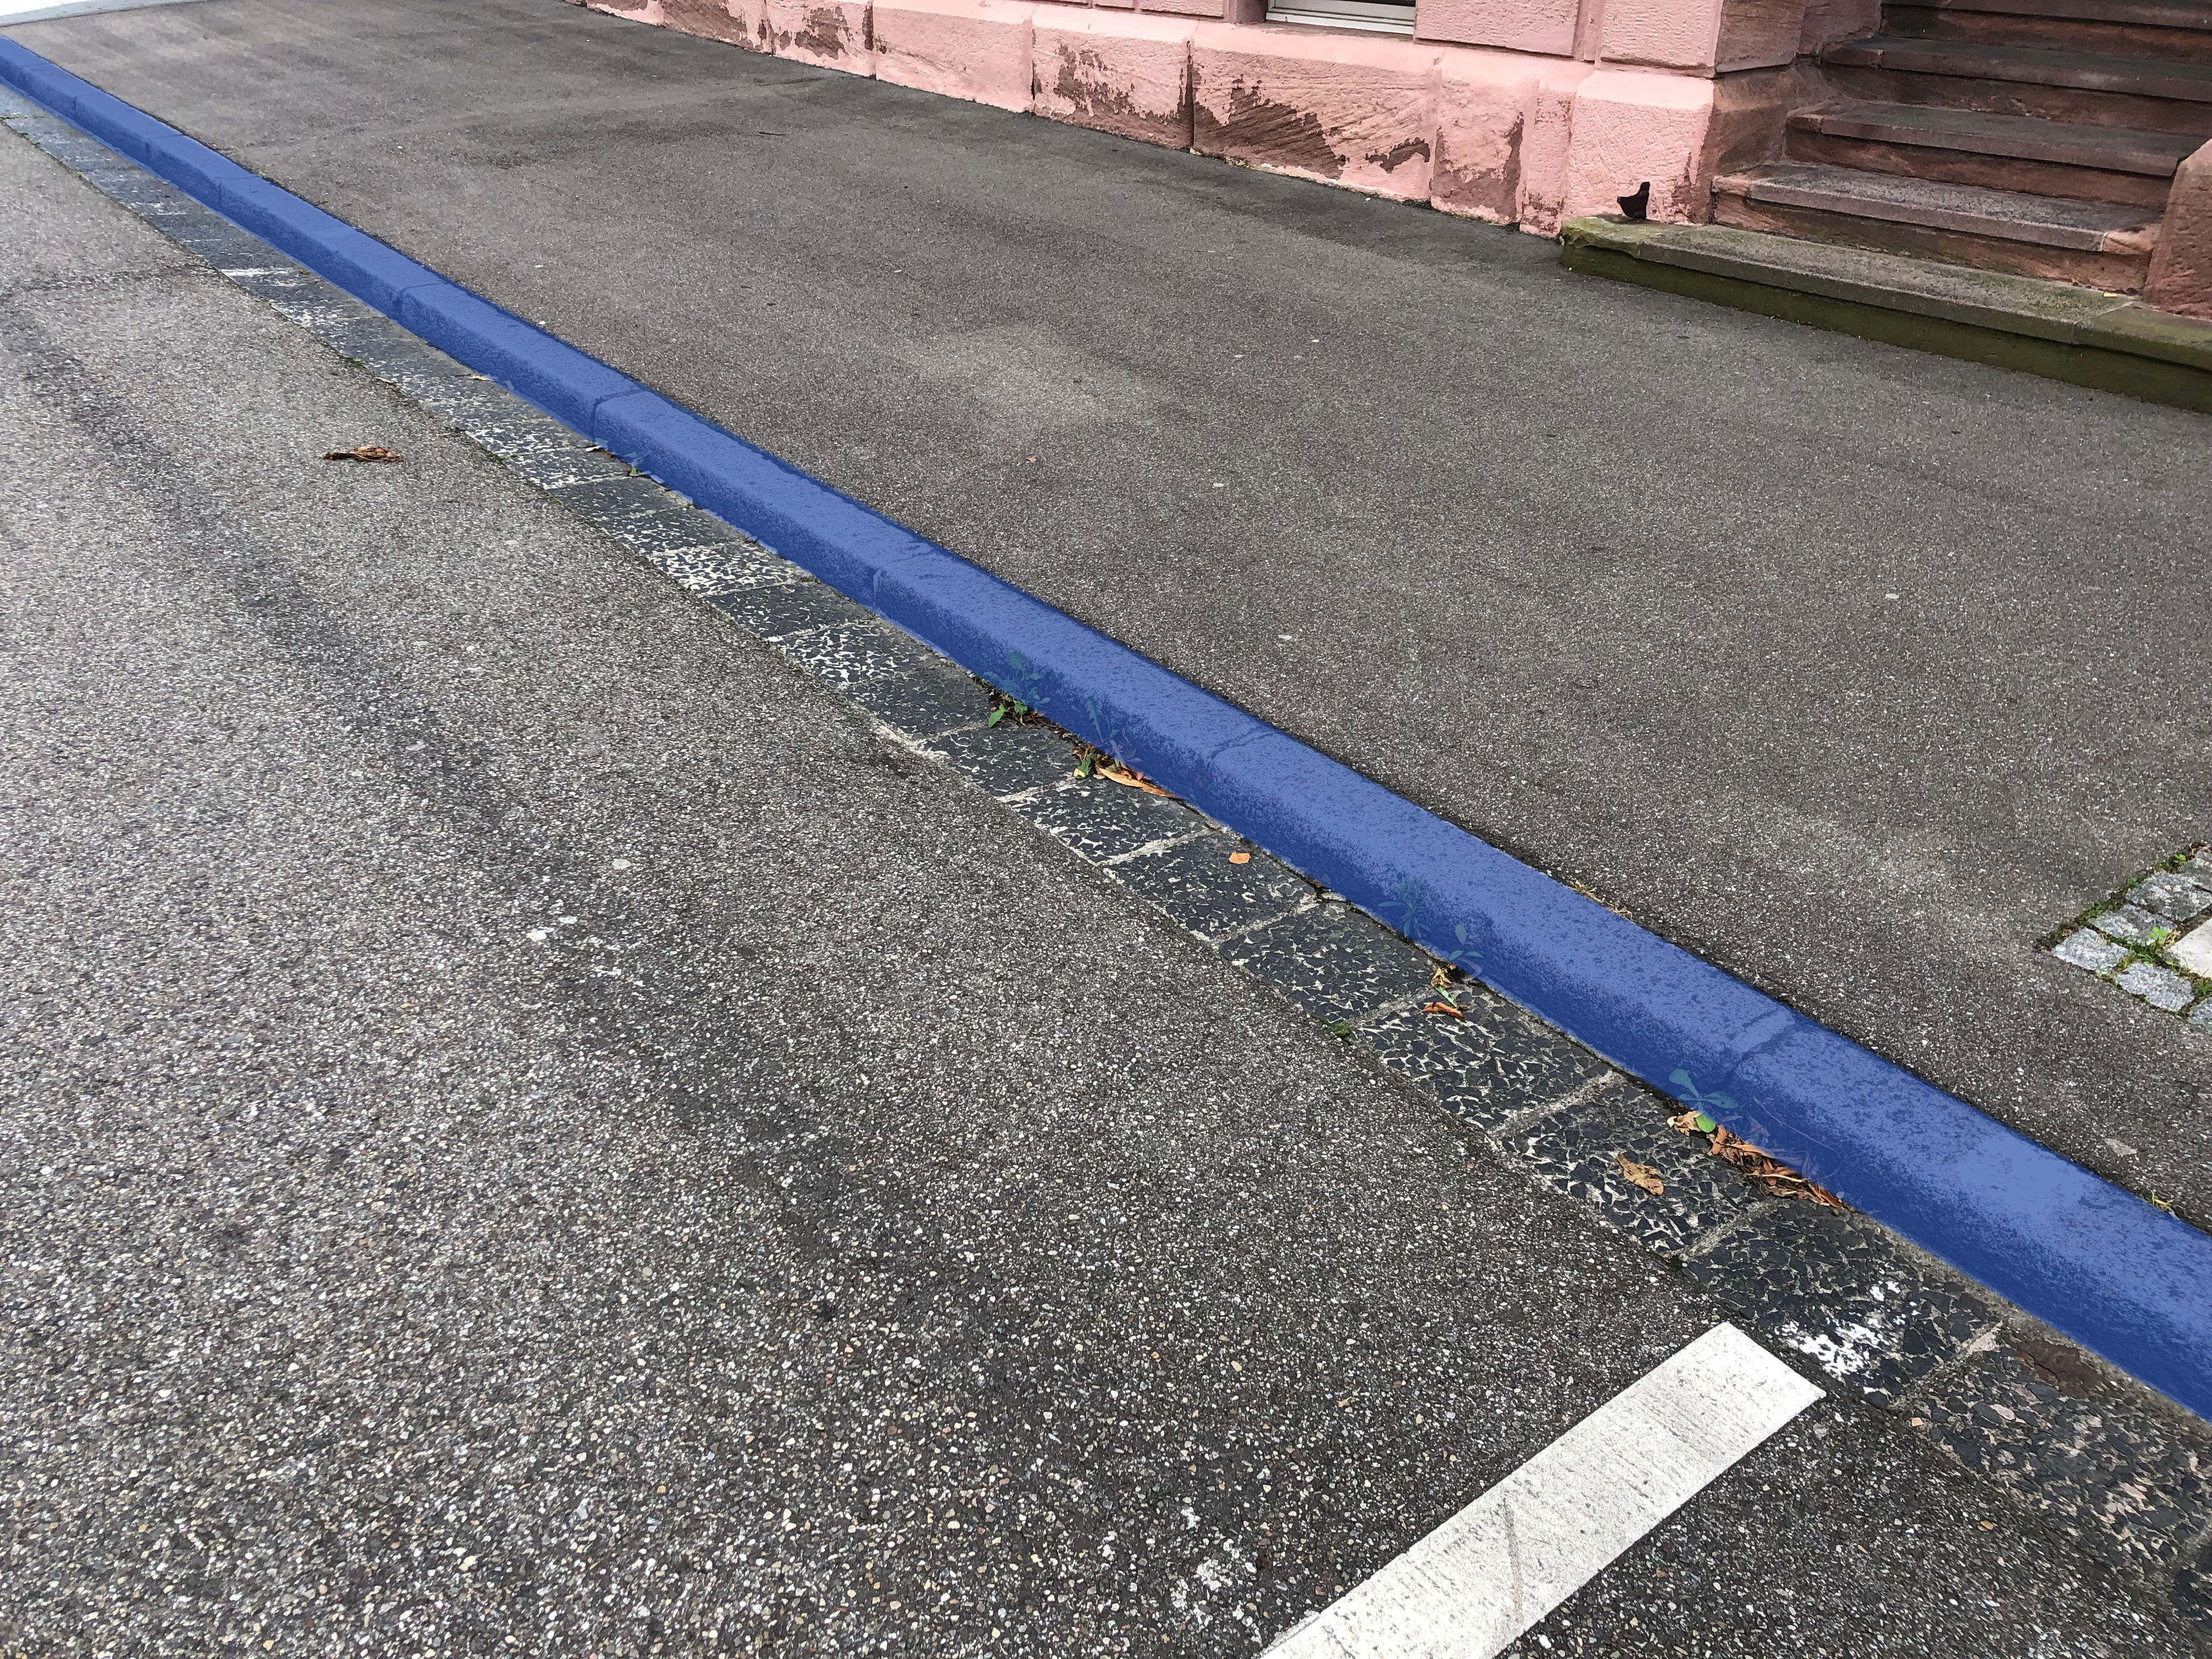
\includegraphics[width=0.9\textwidth]{figures/background/curb.jpeg} % first figure
    	\caption{An example of a sidewalk with a curb, the curb highlighted in blue.} \label{fig:background-curb}
    \end{subfigure}
	\hfill
    \begin{subfigure}{0.45\textwidth}
        \centering
        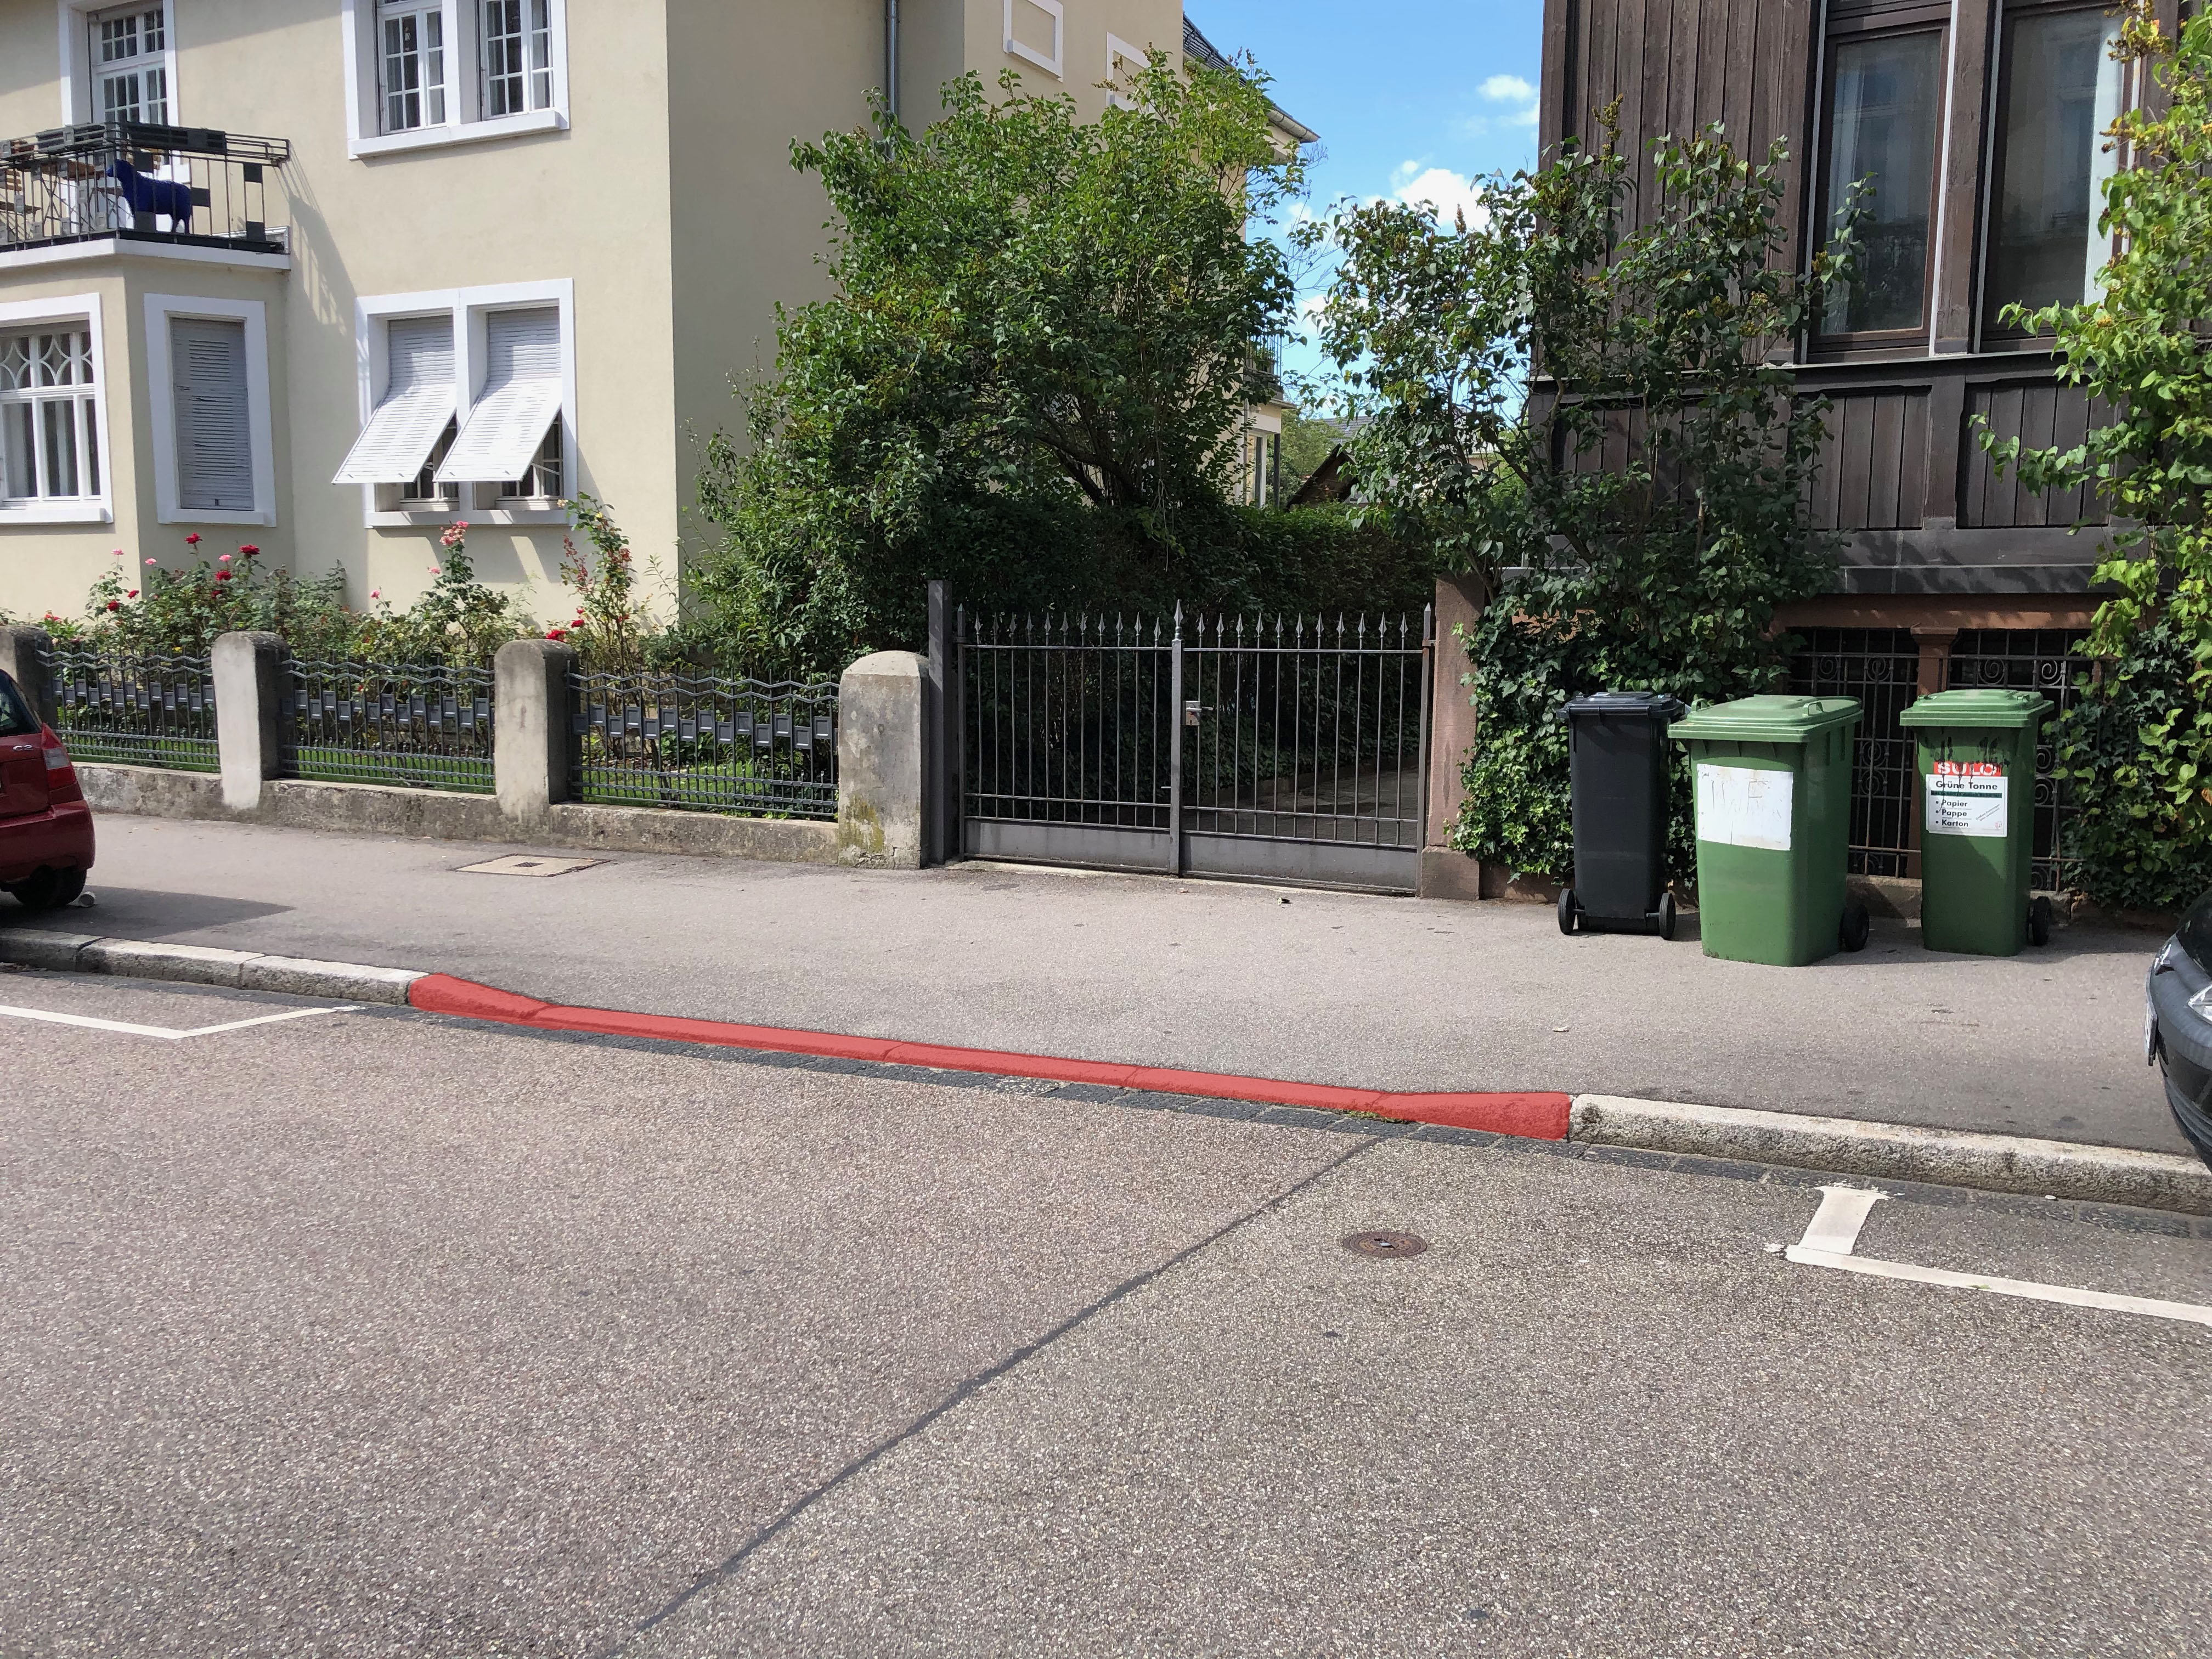
\includegraphics[width=0.9\textwidth]{figures/background/curbcut.jpeg} % second figure
        \caption{An example of a sidewalk with a curb cut, the curb cut highlighted in red.} \label{fig:background-curbcut}
    \end{subfigure}
	\caption[Curbs and curb cuts]{An example of a curb and a curb cut.}
\end{figure}

\section{Loss Functions}\label{section:background-loss}
The loss function $\ell$ maps the output of a neural network $\hat{y}$ and the target $y$ onto a real number and represents the "cost" of an output.
The goal of learning is to minimize this cost value.
Effectively, the loss function measures the difference between the predicted value and the target.
In our case, the target value is the ground truth labeling of an image and the output is the softmax class predictions from the network.
There are many different loss functions that are commonly used. For the purposes of image segmentation, the most commonly used function is cross entropy loss.

\subsection{Cross Entropy Loss}\label{section:background-crossentropy}
The cross entropy loss is formally defined as:
\begin{align}
	\ell(y, \hat{y}) &=\sum_{m}-y_m\log(\hat{y}_m)
\end{align}
where $m$ is the class, $y_m$ the ground truth value for a class $m$, and $\hat{y}_m$ the softmax prediction of a class $m$ by the model. 
As such, cross entropy loss calculates the error of the model to classify a certain value correctly.
The loss of two predictions could be the same, as long as the prediction for the true class, i.e. the class that has value 1 in $y$, remains constant.
The loss is thus independent of how the probability is split between the remaining classes.

For example, let the ground truth classification be class 0, i.e. $y = \{1, 0, 0\}$ with one-hot encoding.
Let the current model prediction be $\hat{y} = \{0.5, 0.2, 0.3\}$, also with one-hot encoding.
The loss would then be:
\begin{equation}
	\begin{split}
		\ell(y, \hat{y}) 	&= \sum_{m}-y_m \log(\hat{y}_m) \\
		&= -(1)\log(0.5) + (-0)\log(0.2) + (-0)\log(0.3)\\
		&= -\log(0.5) \\
		&= 0.301...
	\end{split}
\end{equation}
Alternatively, if model prediction is exactly the same as the ground truth, then we would have:
\begin{equation}
	\begin{split}
		y					&= \hat{y} = \{1, 0, 0\}\\
		\ell(y, \hat{y}) 	&= \sum_{m}-y_m \log(\hat{y}_m) \\
		&= -(1)\log(1) + (-0)\log(0) + (-0)\log(0)\\
		&= -\log(1) \\
		&= 0
	\end{split}
\end{equation}
Applying this on the full image, this becomes:
\begin{align}
	\ell(y, \hat{y}) &=\sum_u \sum_v \sum_{m}-y_{m, u, v}\log(\hat{y}_{m,u,v})
\end{align}
where $u$ and $v$ are the pixel coordinates.

The weighted variant, known simply as weighted cross entropy loss, is defined as:
\begin{align}
	\ell(y, \hat{y}) &=\sum_{m}-y_m\log(\hat{y}_m) \cdot d_m
\end{align}
where $d_m$ is the weight for a given class $m$.

Using the weighted version allows changes to how much each class contributes to the loss.
This is done to counteract class imbalance that could be caused by having an imbalance in the distribution or frequency of each class in the dataset.

\section{Optimizers}\label{section:background-optimizers}
During training, network parameters must be updated to minimize the loss function at each iteration.
This is done by the optimizer.
The optimizer updates the network parameters in such a way as to minimize the loss function~\cite{optimizer-intro}.

Gradient Descent is one of the earliest optimizers.
It works by calculating what a small change in each network parameter would do to the loss function, i.e. determines the gradient of the loss for the current iteration.
It then adjusts the network parameters according to this gradient.
This process is repeated at each iteration to further minimize the loss function.
This process can be time-consuming, especially with larger datasets.
Stochastic Gradient Descent (SGD) is a more commonly used variant of gradient descent and works similarly, but working only on randomly selected batches of the training data at each iteration~\cite{optimizer-intro}.
Due to the large size of datasets, training is usually done in batches.
By using SGD, the optimization step can occur after processing every batch, rather than after the entire dataset is processed.
This speeds up with respect to wall-clock time network training.

Adaptive Moment Estimation (Adam) is another optimizer that is commonly used and first proposed in the paper "Adam: A method for stochastic optimization" by Diederik Kingma and Jimmy Ba~\cite{adam}.
It combines concepts from Adaptive Gradient Algorithm (AdaGrad), which has per-parameter learning rates, and Root Mean Square Propagation (RMSProp), whose learning rates are adapted based on the average of the magnitude of recent gradients~\cite{adam}.
Adam utilizes the concept of momentum, which incorporates previous gradients into the current one.
It does this by calculating an exponential moving average and the square of previous gradients and using these to determine the next gradient.

\section{Backpropagation}\label{section:background-backpropagation}
Backpropagation is a learning procedure used in artificial neural networks to adjust network weights and produce internal representations of "important features in the task domain," first described in 1986 by David E. Rumelhart, Geoffrey E. Hinton, and Ronald J. Williams in their paper "Learning representations by back-propagating errors"~\cite{backprop}.
Backpropagation efficiently and repeatedly adjusts the network weights to minimize the network error, which is calculated by the loss function.

Calculating the network weights is done layer by layer, starting with the final output layer.
The partial derivative of $\ell$ with respect to $y_j$, intuitively the effect the output unit has on the loss, is defined as:
\begin{align}\label{eq:loss-1}
	\frac{\partial \ell}{\partial y_j}
\end{align}
where $y_j$ is the output of a single unit in the final layer.
The contribution of the input of the unit $j$ on the error can then be calculated using the value previously calculated in \eqref{eq:loss-1} using the chain rule for differentiation as
\begin{align}\label{eq:loss-2}
	\frac{\partial\ell}{\partial x_j} &= \frac{\partial \ell}{\partial y_j} \cdot \frac{\partial y_j}{\partial x_j}
\end{align}
We now have a description of how changing the input of unit $j$ will affect the loss.
As such, we can then also represent how changing the weight $w_{ji}$ of a connection between the unit $j$ and a unit in the previous layer $i$ will effect the error as
\begin{align}\label{eq:loss-3}
	\frac{\partial \ell}{\partial w_{ji}} &= \frac{\partial \ell}{\partial x_j} \cdot \frac{\partial x_j}{\partial w_{ji}}
\end{align}
In this case, the previous layer means the layer which during forwards-propagation would be calculated immediately before the layer in which unit $j$ is.
Again, due to the use of the chain rule, the previous value calculated in \eqref{eq:loss-2} can be used here.
This gives us the contribution of the weight $w_{ji}$ on the error and, by multiplying by the learning rate, the amount by which the gradient must be changed for the next training iteration.

The error contribution of the output of unit $i$ via a single successor unit $j$ can also similarly be calculated using the value from \eqref{eq:loss-2}.
\begin{align}\label{eq:loss-4}
	\frac{\partial \ell}{\partial y_i} &= \frac{\partial \ell}{\partial x_j} \cdot w_{ji}
\end{align}
Since unit $i$ is connected to multiple successor units, its value is a summation of its output contribution via all units $j \in J$, where $J$ is the set of all units in successive layers that $i$ is connected to.
\begin{align}
	\frac{\partial \ell}{\partial y_i} &= \sum_{j \in J} \frac{\partial \ell}{\partial x_j} \cdot w_{ji}
\end{align}
This calculation can be done in parallel, thanks to parallel computing architecture, completing the gradient calculations for the penultimate layer.
This procedure is then repeated for all layers, each time using the previously computed values to allow for efficient computation.

\section{Hyperparameter Tuning}\label{section:background-hyperparameter}
Hyperparameter tuning is the process of optimizing a model to find the hyperparameters that will perform optimally given a specified metric. This metric is usually either the validation loss or the validation accuracy.
Hyperparameters are generally chosen by hand or by some automated process, but are not learned as a part of the model itself as opposed to the model weights.

Methods to find the optimal hyperparameters include manual tuning, grid search, random search, genetic algorithms, bayesian optimization, and hyperband, among others.
Random and grid searches are very time-consuming and computationally expensive, as they potentially run less than optimal parameters and do not use knowledge of previous runs to select the next set of parameters.
Bayesian optimization attempts to curtail this problem by taking previous runs into account, greatly speeding up the learning process and not experimenting with less than optimal hyperparameters~\cite{bayesian}.
Hyperband is a bandit-based approach to hyperparameter optimizations that can abandon or reduce the budget of an experimental run if the network performance is below with a chosen parameter set is below a certain threshold~\cite{hyperband}.

\subsection{Bayesian Optimization}\label{subsection:background-bayesian}
The idea behind Bayesian optimization is that the hyperparameters of a network follow a probabilistic distribution $\text{P}(y | x)$ where $y$ is the score determined by some objective function and $x$ is a set of hyperparameters.
Based on this probabilistic model, an optimal set of hyperparameters can then be calculated.
Applying these hyperparameters to the model, the objective function can then be used to calculate the scores.
The probabilistic distribution is then updated and the process is repeated until the maximum number of iterations is reached.

Bayesian optimization relies on the following~\cite{bayesiantds}:
\begin{enumerate}
	\itemsep-1em
	\item A clearly defined hyperparameter domain of possible configurations $\chi$ over which to search,
	\item An objective function which calculates a score that we wish to minimize using a set of hyperparameters,
	\item A surrogate model that represents the probabilistic distribution of the hyperparameters,
	\item A selection function to evalute which hyperparameters should be evaluated next, and
	\item A history of score-hyperparameter pairs used to update the surrogate model.
\end{enumerate}
The domain must be chosen by the researcher and is usually defined with respect to previous knowledge or based on related works.
The objective function is evaluated by running the model and calculating its error using a predetermined loss function.

The surrogate model used is essentially a mapping of hyperparameters to scores from the objective function.
An example for the surrogate model is the Tree-structured Parzen Estimator (TPE)~\cite{tpe}.
TPE takes advantage of Bayes' rule and represents the probability function $\text{P}(y~|~x)$ as
\begin{equation}\label{eq:bohb-1}
	\begin{split}
		\text{P}(y~|~x) &= \frac{\text{P}(x~|~y) \cdot \text{P}(x)}{\text{P}(y)}\\
		\text{with } \text{P}(x~|~y) &=
		\begin{cases}
		l(x) &\text{when } y < y^* \\
		g(x) &\text{when } y \geq y^*
		\end{cases}
	\end{split}
\end{equation}
where $y^*$ is a threshold value. $l(x)$ is thus a probability density function formed from the set of observations using hyperparameters $x^i \in \chi$ which have been performed such that the loss of the network is less than $y^*$. 
Conversely, $g(x)$ is the density function formed from the remaining observations.
$y^*$ is chosen by the algorithm such that $\text{P}(y<y^*) = \gamma$ with $\gamma$ being a value chosen by the researcher.

The selection function chooses which hyperparameters $x \in \chi$ should be chosen for each successive experiment and is commonly based on the expected improvement~\cite{bayesiantds}:
\begin{align}
	EI_{y^*}(x) &= \int_{-\infty}^{y^*} (y^* - y) p(y~|~x)dy
\end{align}
Here, $y^*$ is again a threshold value, $x$ is the proposed set of hyperparameters, $y$ is the actual value of the objective function using hyperparameters $x$ and $p(y~|~x)$ is the surrogate probability model expressing the probability of $y$ given $x$.
Substituting the values of $p(y~|~x)$ from the surrogate function we get
\begin{equation}
	\begin{split}
		EI_{y^*}(x) &= \frac{\gamma y^* l(x) - l(x) \int_{-\infty}^{y^*}p(y)dy}{\gamma l(x) + (1 - \gamma)g(x)}\\
		&\propto \left(\gamma + \frac{g(x)}{l(x)} (1 - \gamma)\right)^{-1}
	\end{split}
\end{equation}
We can see from this function that the expected improvement is proportional to $\frac{l(x)}{g(x)}$ and thus, to maximize the expected improvement, samples should be drawn from the maximum value in $l(x)$.
The selected hyperparameters are then evaluated with regards to the objective function and the results used to update the surrogate model.

\subsection{Hyperband}\label{section:background-hyperband}
Hyperband is a learning strategy that "relies on a principled early-stopping strategy to allocate resources"~\cite{hyperband}. 
It is a variation of successive halving, and in fact uses successive halving in its inner loop~\cite{successivehalving}.

Successive halving randomly samples $n$ hyperparameter sets in the search domain $\chi$.
It then evaluates all of these sets for $B$ iterations to calculate the validation loss.
The lowest performing half is then discarded and the remaining evaluated for a further $B$ iterations.
This is repeated until only one hyperparameter set remains.

Successive halving suffers from the $n \text{ vs } \frac{B}{n}$ problem, which is whether to train more configurations $n$ or to explore fewer, but with more resources $B$.
If a larger $n$ is chosen, configurations which are slower to converge might be killed off too quickly.
If a larger $\frac{B}{n}$ is chosen, then lower performing configurations may be given more resources, thus wasting resources that could otherwise be spent on higher performing configurations~\cite{hyperband}.

Hyperband attempts to solve this issue by considering several possible values of $n$ for a fixed $B$.
The pseudocode in Algorithm \ref{algorithm:hyperband} shows how Hyperband uses an outer loop, performing essentially a grid search with multiple values of $n$ and an inner loop utilizing a method similar to successive halving but with the top $\left\lfloor n_i/\eta\right\rfloor$ instead of the top half.

\begin{algorithm}
	\caption{\textsc{Hyperband} algorithm for hyperparameter optimization}\label{algorithm:hyperband}

	\SetKwInOut{Input}{Input}
	\SetKwInOut{Output}{Output}
	\SetKw{Initialize}{Initialize}
	
	\Input{$R,~\eta~ (\text{default} \eta = 3$)}
	\Output{Configuration with the smallest intermediate loss seen so far.}
	\Initialize{$s_{max} = \left\lfloor \log_\eta(R)\right\rfloor$, $B=(s_{max} + 1)R$}
	
	\For{$s \in s_{max}, s_{max} - 1,...,0$}{
		$n = \left\lceil \frac{B}{R} \frac{\eta^s}{(s+1)}\right\rceil$\\
		$r = R\eta^{-s}$\\
		$T = $ get\_hyperparameter\_configuration$(n)$\\
		\For{$i \in \{0,...,s\}$}{
			$n_i = \left\lfloor n \eta^{-i}\right\rfloor$ \\
			$r_i = r \eta^i$ \\
			$L = $\{run\_then\_return\_validation\_loss$(t,r_i) : t \in T$\}\\
			$T = $top\_k$(T,L, \left\lfloor n_i / \eta \right \rfloor)$\\
		}
	}
\end{algorithm}

\subsection{Bayesian Optimization with Hyperband}\label{section:background-bohb}
"BOHB: Robust and Efficient Hyperparameter Optimization at Scale" by Stefan Falkner, Aaron Klein, and Frank Hutter proposes a hyperparameter optimization approach which seeks to combine the benefits of both Bayesian optimization and Hyperband~\cite{bohb}.
This approach seeks to have strong anytime performance, strong final performance, effectively use parallel resources, be easily scalable, and be robust and flexible.

BOHB works by using Hyperband to determine the number of configurations to evaluate with a given budget, but replaces the random selection of configurations with a Bayesian model based search.
The process of using Bayesian optimization for configuration sampling can be seen in Algorithm \ref{algorithm:bohb}. In this algorithm, $l'(x)$ is the $l(x)$ component of the newly updated probability density function.

Even though Hyperband also provides strong anytime performance compared to random search and Bayesian optimization, Fakner et al. observed an improvement of over 55x against a random search at larger budgets, converging to the global optimum much faster than either Hyperband or Bayesian optimization alone~\cite{bohb}.

\begin{algorithm}
	\caption{\textsc{BOHB} algorithm for hyperparameter optimization}\label{algorithm:bohb}

	\SetKwInOut{Input}{Input}
	\SetKwInOut{Output}{Output}
	\SetKw{Initialize}{Initialize}
	
	\Input{observations $D$, fraction of random runs $\rho$, percentile $q$, number of samples $N_s$, minimum number of points $N_min$ to build a model, and bandwidth factor $b_w$}
	\Output{next configuration to evaluate}
	
	\If{rand() $< \rho$}{
		\Return{random configuration}
	}
	$b = \text{arg max }\{D_b:|D_b|\geq N_min + 2\}$\\
	\If{$b=\emptyset$}{
		\Return{random configuration	
	}}
	fit P$(x~|~y)$ according to \eqref{eq:bohb-1}\\
	draw $N_s$ samples according to $l'(x)$\\	
	\Return{sample with highest ratio $l(x) / g(x)$}
\end{algorithm}

\section{Binary Dilation}\label{section:background-dilation}
Binary dilation is a basic morphological operation and is usually represented by the operator $\oplus$.
With regards to this work, binary dilation is used in our loss function.
For a given binary image viewed as an integer grid $\mathbb{Z}^d$ for some dimension $d$, let $E$ be an integer grid, $A \in E$ a binary image, and $B \in \{0,1\}^d$ a structuring element.
The binary dilation of $A$ by $B$ is then defined as:
\begin{align}
	A \oplus B &= \bigcup_{b \in B}A_b
\end{align}
where $A_b$ is the translation of $A$ by $b$.
This can be seen as extending the area of the binary image $A$ by locus of the points covered by $B$ given that $B$ has a center on the origin~\cite{morphology}.